\subsection*{Actividad 2}

\begin{center}
Consumo de heladeras en vatios por hora, según eficiencia\\
\vspace{4mm}
\begin{tabular}{ccccc}
Horas & A     & C   & D   & E   \\ \hline
0     & 0     & 0   & 0   & 0   \\
1     & 26.5  & 41  & 50  & 59  \\
2     & 53    & 82  & 100 & 118 \\
3     & 79.5  & 123 & 150 & 177 \\
4     & 106   & 164 & 200 & 236 \\
5     & 132.5 & 205 & 250 & 295 \\
6     & 159   & 246 & 300 & 354 \\ \hline
\vspace{5mm}
\end{tabular}
\end{center}

Gráficamente:

\begin{center}
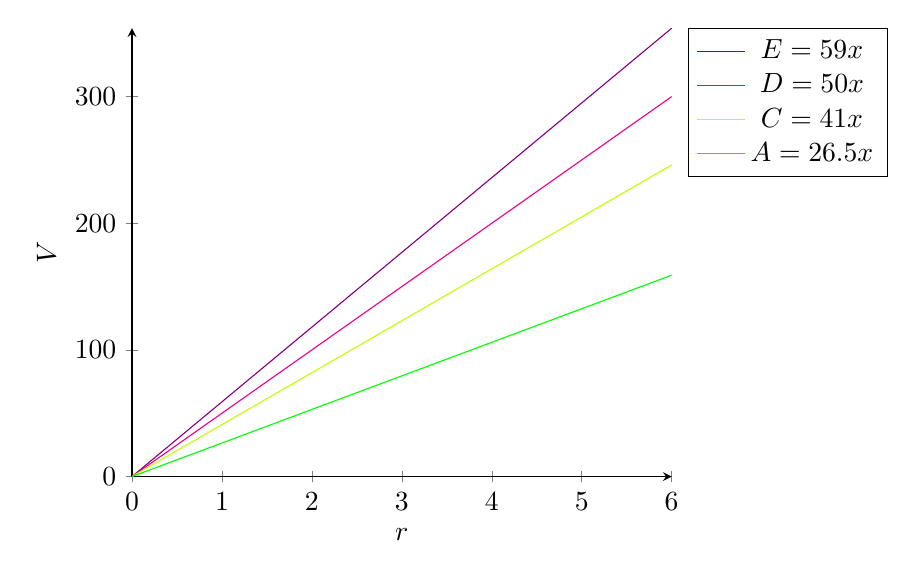
\begin{tikzpicture}
\begin{axis}[
    axis lines = left,
    xlabel = \(r\),
    ylabel = {\(V\)},
    clip = false,
    legend pos = outer north east,
    ymin = 0,
    xmin = 0,
]

% E
\addplot [
    domain=0:6, 
    samples=200, 
    color=violet,
]
{59 * x};
\addlegendentry{\(E = 59x\)}

% D
\addplot [
    domain=0:6, 
    samples=200, 
    color=magenta,
]
{50 * x};
\addlegendentry{\(D = 50x\)}

% C
\addplot [
    domain=0:6, 
    samples=200, 
    color=lime,
]
{41 * x};
\addlegendentry{\(C = 41x\)}

% A
\addplot [
    domain=0:6, 
    samples=200, 
    color=green,
]
{26.5 * x};
\addlegendentry{\(A = 26.5x\)}

\end{axis}
\end{tikzpicture}
\end{center}

Las función de consumo de cada categoría de heladera es:

\begin{align*}
	A(h) &= 26.5h\\ 
	C(h) &= 41h\\ 
	D(h) &= 50h\\ 
	E(h) &= 59h
\end{align*}

La pendiente de cada función indica el consumo en vatios por hora de cada categoría de heladera.

Una heladera de eficiencia A consume 636 vatios por día, mientras una heladera de eficiencia E consume 1416 vatios por día. Usar una heladera de tipo A permite ahorrar hasta un 55\% de vatios al día.

